\documentclass[12pt,a4paper]{article}
\usepackage[utf8]{inputenc}
\usepackage{amsmath}
\usepackage{amsfonts}
\usepackage{amssymb}
\usepackage{graphicx}
\usepackage{tikz}
\usetikzlibrary{automata, positioning, arrows}

\title{Notas de conferencias}
\author{Sherlyn Ballestero Cruz \\ Maria de Lourdes Choy Ferna\'ndez}

\begin{document}
\maketitle
\newpage
\pagestyle{myheadings}
\markright{Introdicci\'on a la Teor\'ia de lenguajes y Aut\'omatas}
\textit{Conferencia2}\\
\textbf{Alfabeto:} Conjunto de s\'imbolos.\\
\textbf{Secuencia de s\'imbolos:} conjunto que contiene un s\'imbolo y una secuencia de s\'imbolos.\\
\textbf{Cadena:} secuencia de s\'imbolos con cierto orden.\\
\textbf{Vocabulario sobre un alfabeto $V^{*}$:} todas las posibles cadenas dado un alfabeto V.\\
\textbf{Lenguaje sobre un alfabeto:}Subconjunto del vocabulario sobre un alfabeto  ,$L \subseteq V
$.(Se le pueden aplicar todas las definiciones estudiadas en \'algebra de conjunto).\\
Se tienen lenguajes como  el lenguaje de todas las cadenas que representan el resultado a determinado problema.Esto  permite determinar que cierto problema no tiene soluci\'on dado que dicho lenguaje es una referencia negada.\\
\textbf{Problema de la palabra:}
Teorema fundamental en la teor/'ia del lenguaje, consiste en dado una cadena w que pertenece al vocabulario saber si esta pertenece al lenguaje L.\\
Ejemplo de ello es un lenguaje en el que se encuentre dado un array, su array ordenado, si este fuese el vacio ser\'ia evidente que el problema a resolver(ordenaci\'on) no tiene soluci\'on, de otro modo, si hubiesen elementos(que los hay), dado una permutaci\'on cualquiera de un array si esta pertenece al lenguaje entonces est\'a ordenada.\\
\textbf{Lenguajes decidibles o computables:}
Son aquellos para los cuales el problema de la palabra siempre tiene soluci\'on, hay un algoritmo.\\
\textbf{aut\'omata:}
Mecanismo abstracto que representa un proceso de c\'omputo, podemos verlo como una maquinita reconocedora.Este recibe una cadena y la analiza s\'imbolo a s\'imbolo \\
Un aut\'omata puede verse como un conjunto de estados y un conjunto de instrucciones que determinan, dado un estado del aut\'omata, y un s\'imbolo de la cadena que est\'a siendo "analizado", cu\'al es el nuevo estado del aut\'omata y cuando el estado final coincide con determinados estados esta devuelve True.\\
\textbf{Aut\'omata finito determinista:}Un FDA es un aut\'omata con un conjunto finito de estados que "lee" la cadena de inicio a fin una sola vez y tiene que tomar una decisi\'on, aceptar o rechazar la cadena.\\
Formalemente es una tupla:
$A=<V,Q,q_{0},F,f>$, donde V es un alfabeto de entrada, Q un conjunto de estados, F un subconjunto de estados finales y f una funci\'on de transici\'on,$ VxQ->Q$.
\\
\textbf{>C\'omo funciona un FDA?}\\
Dado una cadena $ w \in V^{*}$, empezando por el estado $q_{0}$, por cada s\'imbolo perteneciente a w se le aplica la funci\'on f hasta llegar al final de la cadena, donde nos encontramos con un estado final que si pertenece a F entonces el algoritmo retorna true o se acepta y false en caso contrario, si en alg\'un punto la funci\'on de transici\'on no est\'a definida el aut\'omata se traba y no se acepta.\\
El lenguaje de un FDA cualquiera,L(A) es el lenguaje $L\subseteq V^{*}$ tal que toda cadena $w\in L(A)$ es aceptada por el autómata.\\
A continuaci\'on como ejemplo el 'Hello World!' de los aut\'omatas!!:\\
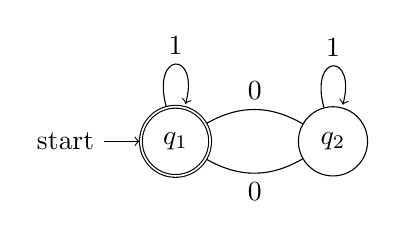
\begin{tikzpicture}
\node[state, initial,accepting] (q1) {$q_1$};
\node[state, right of=q1,xshift=1cm] (q2) {$q_2$};
\draw (q1) edge[loop above] node{1} (q1)
(q2) edge[bend right,above] node{0}(q1)
(q1) edge[bend right, below] node{0} (q2)
(q2) edge[loop above] node{1} (q2);
\end{tikzpicture}
\\Aqui se analiza si una cadena cualquiera, a partir del alfabeto $V={0,1}$, tiene una cantidad par de 0.\\
El estado inicial es $q_{1}$ y el conjunto de estados finales aceptados es $F={q_{1}}$, donde f es la funci\'on en la que si el estado actual es $q_1$ y el siguiente s\'imbolo es 1 entonces pasa a $q_{1}$ y si es 0 este pasa al estado $q_2$, si el estado actual es $q_{2}$ y el siguiente s\'imbolo es 0 entonces pasa a $q_{1}$ y si es 1 entonces se queda en $q_{2}$ .  



 




\end{document}